\documentclass[times, utf8, seminar, numeric]{fer}
\usepackage{booktabs, url, hyperref}
\usepackage{verbatim}
\usepackage{moreverb}
\usepackage{subfigure}
\usepackage{caption}
\usepackage{epstopdf}
\usepackage{amsthm}
\usepackage{graphicx}
\usepackage{caption}
\usepackage{subcaption}

\hypersetup{
   colorlinks,
   citecolor=black,
   filecolor=black,
   linkcolor=black,
   urlcolor=black
}

%dodatak za programski kod
\usepackage{listings}
\usepackage{color}
\usepackage{setspace}
\definecolor{dkgreen}{rgb}{0,0.6,0}
\definecolor{gray}{rgb}{0.5,0.5,0.5}
\definecolor{mauve}{rgb}{0.58,0,0.82}

\lstset{frame=tb,
  language=Java,
  aboveskip=3mm,
  belowskip=3mm,
  showstringspaces=false,
  columns=flexible,
  basicstyle={\small\ttfamily},
  numbers=left,
  numberstyle=\small\color{gray},
  keywordstyle=\color{blue},
  commentstyle=\color{dkgreen},
  stringstyle=\color{mauve},
  breaklines=true,
  breakatwhitespace=true,
  tabsize=2
}


\begin{document}

% TODO: Navedite naslov rada.
\title{Histogram orijentiranih gradijenata - detekcija i praćenje ljudi}

% TODO: Navedite vaše ime i prezime.
\author{Petra Bevandić \\ Dragan Drandić \\ Melita Kokot \\ Igor Smolkovič \\ Dino Šantl}

\maketitle

\tableofcontents

\chapter{Projektni zadatak}
\section{Opis projektnog zadatka}
Razvoj informatičke tehnologije omogućio je primjenu računala na kompleksnim problemima poput analize i razumijevanja sadržaja slike i doveo do razvoja područja računalnog vida. Dva goruća problema u računalnom vidu jesu detekcija objekata u slikama, odnosno praćenje objekata u videosekvencama. Oba ova problema svoju primjenu pronalaze u nizu područja, od video nadzora, navigacije, pretraživanja sadržaja pa sve do naknadne obrade videosekvenci.

U sklopu ovog projekta objekti koje je trebalo detektirati i pratiti u video snimkama bili su ljudi. Da bi to bilo moguće, bilo je potrebno implementirati sustav za ekstrakciju značajki iz slika koje su prikladne za opis slika koje sadrže ljude (odabran je histogram orijentiranih gradijenata), zatim odgovarajući klasifikator koji te značajke koristi (te naučiti model za prepoznavanje osoba) te sustav za praćenje kretanja objekata u nekom video zapisu.  Dodatno, bilo je potrebno usporediti uspješnost primjene histograma orijentiranih gradijenata za opis osoba s drugim popularnim značajkama (konkretno Haarovskim značajkama koje koristi Viola-Jones).

U nastavku rada daje se pregled radova na kojima se temelji implementirani sustav, zatim  se iscrpno opisuju svi koraci rada sustava i konačno, daju se pregled i analiza efikasnosti naučenog klasifikatora te rezultati rada cjelokupnog sustava na odabranim videosnimkama.  Ovi su rezultati uspoređeni s rezultatima detektora osoba temeljenog na Viola-Jones algoritmu. Na kraju se daje analiza ovih rezultata i moguća poboljšanja implementiranog sustava.

\section{Pregled i opis srodnih rješenja}
Histogram orijentiranih gradijenata prvi je put opisan i korišten za detekciju ljudi u slikama  u \cite{hog}. Rezultati rada pokazuju da histogram orijentiranih gradijenata daje bolje rezultate od drugih značajki poput sifta i haarovskih značajki. Osim toga rad ispituje utjecaj parametara koji se mogu mijenjati prilikom računanja HOG-a na uspješnost pronalaska ljudi u slikama. Smjernice dane u tom radu iskorištene su prilikom izvlačenja značajki iz slika i učenja klasifikatora.

HOG je značajka koja nije otporna na skaliranje tako da se detekcija ljudi vrši pretraživanjem slike korištenjem prozora različitih veličina što može biti vremenski neučinkovito, \cite{fast} predlaže način ubrzanja računanja HOG-a većih prozora korištenjem histograma izračunatih za prozore manjih dimenzija. Konkretna metoda računanja preuzeta je iz \cite{hog1}, koja daje općenitu metodu računanja bilo koje vrste histograma za veće prozore korištenjem histograma manjih prozora. S obzirom da je računanje HOG-a relativno sporo čak i uz ova poboljšanja, pogotovo uzme li se u obzir da je sustav implementiran u Pythonu, ovaj rad koristi drugačiji pristup pretraživanja slike. Ipak, saznanja iz ovoga rada mogu se primijeniti za eventualna poboljšanja implementiranog sustava.

\cite{pedestrian} prikazuje rezultate korištenja HOG-a na infracrvenim snimkama učenjem SVM klasifikatora koja bi imala primjenu u detekciji u praćenju pječaka noću, međutim uspješnost implementiranih sustava je upitna.\cite{enhancing} implementira detektor ljudi u slikama korištenjem HOG-a i koristi već opisano ubrzanje računanja HOG-a. Novost koju uvodi jest da koristi HOG izračunat za prozore manjih dimenzija za računanje HOG-a prozora većih dimenzija, no uz takav odabir prozora koji uvodi Gaussovo zamućenje u prozore većih dimenzija. Ovime se pokušava smanjiti osjetljivost klasifikatora na pomake u orijentaciji osoba, te pokusi pokazuju poboljšanje performansi u odnosu na prethodne radove.

Dok su svi dosad opisani sustavi radili detekciju osoba u slikama, \cite{visual} primjenjuje HOG za detekciju orijentacije vozila u slikama bez znanja o smjeru kretanja vozila (dakle detekciju orijentacije u slikama). Ovo je zapravo klasifikacijski problem gdje je svaka moguća orijentacija jedna klasa. Rad sustava varira o odabiru mogućih orijentacija - radi dobro ukoliko su moguće orijentacije prednja strana, bočna strana koso u odnosu na kameru, no ima problema ukoliko treba razlikovati prednju od stražnje strane ili odlučiti kreće li se vozilo u lijevu ili desnu stranu.

Različite metode praćenja osoba u videosekvencama opisane su u \cite{object}, \cite{realtime}, \cite{efficient} i \cite{fast-accurate}.

Za učenje klasifikatora koji prepoznaje sliku čovjeka na temelju HOG značajki korištena je INRIA baza slika (koja je ujedno korištena i u \cite{hog}. Podijeljena je na pozitivne (na slici se nalazi jedna ili više osoba) i negativne (na slici nema niti jedne osobe). Uz to, baza sadrži i opisnike slike koji u sebi sadrže informacije o pozicijama osoba na slikama (informacija potrebna da bi se iz jedne slike s više osoba izvuklo više slika na kojima se nalazi samo jedan čovjek). Slike su dostupne u više različitih dimenzija: 70x134, 96x160 i 64x128. Baza se sastoji od ukupno 1218 negativnih primjera slika i 614 pozitivnih slika. Za generiranje negativnih primjera, negativne slike mogu se izrezivati na bilo koji način. Nad pozitivnim slikama definirani su opisnici tako da se ukupno može generirati 2500 pozitivnih primjera.

Sam sustav za detekciju i praćenje ispitan je na Caviar Test Case Scenarios bazi video snimaka koja uglavnom sadrži snimke javnih nadzornih kamera. Baza se sastoji od skupa ciljanih akcija osoba. S obzirom da same akcije nisu bile u središtu zanimanja ovog rada, nije postojalo ograničenje na tipove snimki koje je trebalo ispitati.

\section{Konceptualno rješenje zadatka}
Implementirani sustav za praćenje ljudi u video snimkama sastoji se od četiri podsustava: podsustava za ekstrakciju značajki koji kao ulaz prima sliku jednog čovjeka, a na izlazu daje vektor značajki, zatim klasifikatora koji  na ulazu prima vektor značajki, a na izlazu daje odluku o sadržaju slike - slika predstavlja sliku osobe ili slika ne sadrži osobu, podsustava koji unutar slike detektira moguće osobe koji na ulazu prima sliku, a na izlazu daje položaje slike koji potencijalno sadrže osobu i konačno sustava koji u slici detektira otprije detektiranu osobu (na ulazu prima sliku osobe koju se prati te sliku u kojoj je potrebnu tu osobu pronaći, a na izlazu daje označenu osobu).

Konačan sustav koristi sve ove podsustave ne bi li u videosnimci detektirao i pratio osobe. Najprije se unutar pojedine sličice \engl{frame} pronalaze dijelovi slike koji potencijalno sadrže osobu, zatim se iz tih podslika izvlače potrebne značajke koje se šalju klasifikatoru. One podslike za koje klasifikator utvrdi da predstavljaju osobe zatim se prosljeđuju sustavu koji u svim sljedećim sličicama nastavlja pratiti detektirane ljude bez potrebe za ponovnom detekcijom osoba. Detekcija osoba pokreće se svakih nekoliko sličica da bi se omogućila detekcija novih osoba u snimkama. Slike \ref{sustav} i \ref{pozadina} sadrže dijagrame rada cijelog sustava, odnosno podsustava za detekciju objekata.
\begin{figure}
\centering
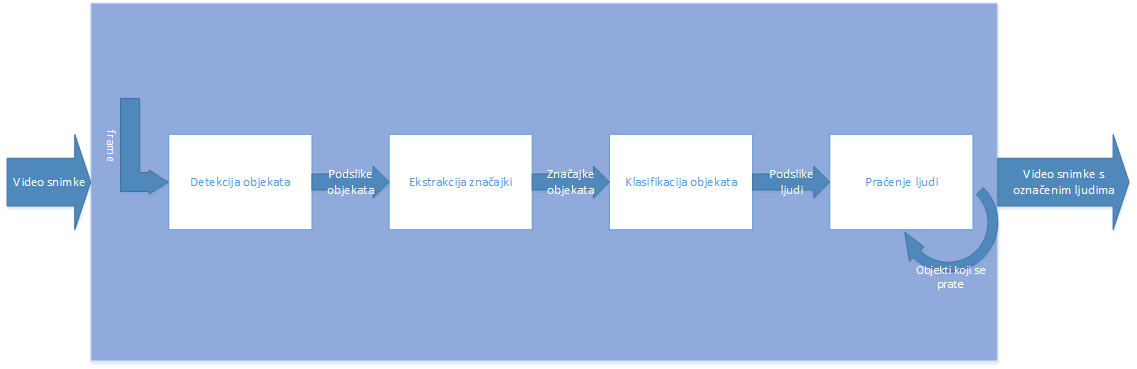
\includegraphics[width=1.1\textwidth]{sustav.png}
\caption{Model sustava}
\label{sustav}
\end{figure}
\begin{figure}
\centering
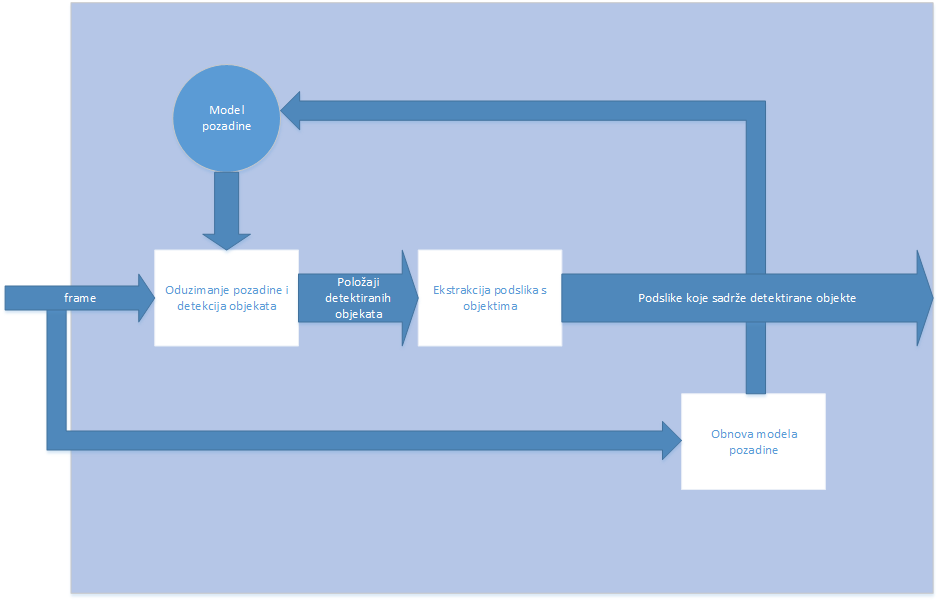
\includegraphics[width=1\textwidth]{pozadina.png}
\caption{Model detekcije objekata}
\label{pozadina}
\end{figure}
U nastavku je detaljno opisan način rada svakog od ovih podsustava i način korištenja svih dijelova u konačnom sustavu.
\chapter{Postupak rješavanja zadatka}
Svi dijelovi sustava implementirani su u programskom jeziku Python uz korištenje OpenCV biblioteke koja sadrži implementacije često korištenih algoritama računalnog vida i strojnog učenja.
\section{Ekstrakcija značajki}
\subsection{Histogram orijentiranih gradijenata}
Histogram orijentiranih gradijenata predstavlja lokaliziranu distribuciju intenziteta gradijenata. Lokalizacija se postiže podjelom slike na ćelije (manje nakupine piksela) te se zatim računa gradijent za svaki piksel unutar ćelije iz čega se zatim radi distribucija smjerova izračunatih gradijenata. Zbog stabilizacije rezultata, ćelije se zatim kombiniraju u blokove za koje se računa ukupna energija lokalnih histograma te se vrijednosti histograma za pojedine ćelije normaliziraju u odnosu na ukupnu energiju bloka. Konačan HOG deskriptor zapravo predstavlja konkatenaciju histograma orijentacija gradijenata pojedinih ćelija unutar svih razmatranih blokova.

Parametri ekstrakcije deskriptora na koje se može utjecati jesu: način računanja gradijenata za pojedini piksel, moguće orijentacije, zatim doprinos pojedinog gradijenta konačnom histogramu, oblik i veličina ćelije te ovisno o odabranoj ćeliji način kombiniranja ćelija u blokove i konačno metoda normalizacije histograma. Način računanja gradijenata odnosi se na odabir maske koja se koristi  za procjenu gradijenata u slici. Pokazalo se da su najbolji rezultati dobiveni za jednodimenzionalne centrirane maske (npr. [1 0 -1]). Što se tiče orijentacija, histogram se može računati ili nad intervalom 0-180  stupnjeva ili na intervalu 0-360 stupnjeva - ovo zapravo znači da se osim smjera gradijenta može promatrati i orijentacija. Jednom kada je definiran interval unutar kojega se nagib gradijenta može nalaziti, potrebno je definirati gustoću podjele tog intervala (s obzirom da konačni deskriptor mora imati konačan diskretan broj značajki). Pokazuje se da su najbolji rezultati u prepoznavanju osoba postignuti ukoliko se ne promatra orijentacija te ako je broj mogućih binova 9. Što se tiče doprinosa samog gradijenta histogramu, on može biti nekakva funkcija iznosa samoga gradijenta. U praksi se najboljom pokazao sam iznos gradijenta. Da bi se neutralizirala činjenica da je originalni interval mogućih smjerova podijeljen u diskretne intervale, gradijent u pojedinom pikselu ćelije uvijek istovremeno doprinosi dvama binovima, dok se sam iznos računa bilinearnom interpolacijom između centara susjednih binova. Sami blokovi mogu dolaziti u dva oblika - pravokutnom i kružnom. Pravokutni blokovi tada sadrže pravokutne ćelije, dok kružni blokovi sadrže ćelije koje nastaju podjelom originalnog kruga bloka u koncentrične krugove koji se dodatno dijele na kružne isječke. Najbolje su performanse detektora postignute za pravokutne blokove veličine 2x2 i 3x3 i veličine ćelije 6x6. Normalizacija se najčešće vrši tako da se svaka vrijednost vektora značajki bloka podijeli nekom normom tog istog vektora.  Potrebno je napomenuti da se blokovi koji se koriste preklapaju, što znači da će pojedini pikseli i ćelije doprinjeti konačnom vektoru značajki kroz više blokova.

Izvlačenje značajki unutar ovog rada vrši se pomoću već gotove openCV funkcije hog koja dopušta isključivo korištenje kvadratnih blokova, uz mogućost definicije veličine blokova i ćelija. Sljedeći \cite{hog1} veličina ćelija postavljena je na 6x6 piksela, dok je veličina blokova postavljena na 3x3 ćelije po bloku. Ono što se može primjetiti jest da ukupan broj blokova, odnosno veličina konačnog HOG deskriptora neke slike ovisi o veličini same slike. S obzirom da treniranje klasifikatora zatjeva da je broj značajki stalan (jednak za sve primjere), u implementaciji je bilo potrebno utvrditi željenu veličinu vektora HOG značajki, a time posredno i fiksirati veličinu slike iz koje se izvlače značajke. Ovo zapravo znači da sustav za ekstrakciju značajki prije samog postupka računanja značajki mora sliku skalirati na neku predefiniranu veličinu (u sklopu ovog projekta ta je veličina postavljena na 128 x 64 piksela).

\section{Klasifikator}
\subsection{SVM}
Stroj s potpornim vektorima predstavlja binarni linearni klasifikator koji pokušava pronaći optimalnu granicu u smislu maksimalne udaljenosti od skupa uzoraka obje klase. Ovu granicu pronalazi detekcijom "potpornih vektora" - onih uzoraka koji su toj granici najbliži te najviše utječu na njezin položaj u prostoru. Optimalna granica tada je ona koja se nalazi na jednakoj udaljenosti od potpornih vektora iz obje klase. Prava snaga SVM-a leži u činjenici da je korištenjem jezgrenih funkcija moguće prijeći u vektorski prostor beskonačnih dimenzija bez potrebe i za stvarnim prelaskom u taj beskonačno dimenzionalni prostor.

I za SVM je korištena gotova implementacija u sklopu OpenCV-ja.

\subsection{Postupak učenja modela}
Postupak učenja modela klasifikatora proveden je nad skupom primjera iz baze slika pješaka INRIA. Baza sadrži slike na kojima se nalazi jedna ili više osoba. Odlučeno je da se klasifikacija slika vrši na dvije kategorije: slika sadrži osobu ili slika ne sadrži osobu. Pritom postoje neke pretpostavke o slici koja sadrži neku osobu - slika sadrži samo jednu osobu, te ta osoba zauzima veći dio slike. Ovo zapravo znači da se ne uče karakteristike slika koje sadrže ljude općenito, već se uči opisnik jedne osobe. Uzevši u obzir ove pretpostavke INRIA bazu je prethodno bilo potrebno pretprocesirati i iz slika koje sadrže više osoba izvući podslike koje sadrže samo jednu osobu te će kasnije predstavljati pozitivne primjere za učenje. S obzirom da ekstraktor značajki sliku skalira na predefiniranu veličinu od 128 x 64 prilikom izrezivanja pojedinih primjera pokušala se obratiti pažnja da izrezane podslike zadržavaju taj isti omjer visine i širine jer bi u suprotnom moglo doći do prevelikih distorzija slike i narušavanja naučenog modela. Da bi se dodatno poveća skup za učenje, svi su ekstrahirani primjeri zrcaljeni oko y osi. Dakle, svaka se slika u skupu  za učenje pojavljuje dva puta - jednom u svom originalnom obliku, a drugi put zrcljena.

Negativni primjeri izvučeni su nasumično iz slika koje sigurno ne sadrže ljude i skalirani na željeni omjer. Iz pozitivnih i negativnih primjera zatim su izvučeni HOG deskriptori koji su zatim proslijeđeni sustavu za učenje modela SVM klasifikatora. Performanse klasifikatora ispitane su na dvije podjele skupa uzoraka na skup za učenje i skup za testiranje - prva u omjeru 50-50, druga u omjeru 70-30. Naučeni modeli su pokazivali vrlo dobre rezultate te nije bilo potrebe za njihovim retreniranjem.

U \cite{hog} predlaže se dodatna metoda poboljšanja rada klasifikatora koja primjere koje je SVM pogrešno naučio u skupu za učenje udvostručuje i tako modificirani skup za učenje koristi u izgradnji konačog modela. Opet, rezultati rada klasifikatora pokazali su da za ovakvim nečim nema potrebe.

\section{Detekcija osoba}
Klasifikator je u mogućnosti samo reći radi li se na slici o osobi ili ne. Da bi se dva prethodna podsustava mogla iskoristiti u analizi kompleksnih scena koje mogu sadržati više osoba, ili osobu u nekom prostoru, potrebno je razviti sustav koji će na neki način sustavno pretraživati tu kompleksnu sliku. Ovo je tim teže uzme li se u obzir ograničenost HOG značajki - one rade isklučivo na slikama predefinirane veličine.

Većina radova opisanih u prvom dijelu rada tom problemu pristupa korištenjem prozora različite veličine. Dakle, krenuvši od manje veličine prozora, njime se kreće po slici te se za svaki pomak iznova računaju HOG-značajke, koje se zatim šalju klasifikatoru. Osim što je potrebno ispitati sve moguće pomake nekog prozora unutar slike, isti je postupak potrebno provesti i za prozore drugih veličina. Kombiniranjem informacija o prozorima u kojima je klasifikator identificirao osobe, moguće je i konačno odrediti područja u slici gdje se te osobe nalaze. Ovakav pristup je vremenski izrazito zahtjevan, te se tom problemu pokušalo doskočiti na razne načine, na najviše se pokušalo ubrzati računanje HOG deskriptora, što predstavlja vremenski najskuplji postupak rada ovog sustava (no čak i uz optimizaciiju zadržava polinomijalnu složenost).

Vremenska zahtjevnost računanja značajki postaje još izraženija uzme  li se u obzira da je implementacija nastala u sklopu ovog projekta ostvarena u programskom jeziku Python. Da bi se ovom problemu doskočilo odlučeno je da će se u detekciji mogućih prozora koji sadrže ljude koristiti informacija koju je moguće saznati iz videosekvenci, ali ne i slika - informaciju o pozadini. Naime, ukoliko je poznata pozadina tada je moguće piksele razvrstati na one koji pripadaju pozadini i one koji joj ne pripadaju. Sve piksele za koje je utvrđeno da ne pripadaju pozadini pokušava se grupirati. Područje slike oko svake od dobivenih grupa zatim se izrezuje, šalje podsustavu za ekstrakciju značajki koje se zatim prosljeđuju klasifikatoru. Ukoliko se za neku podsliku utvrdi da predstavlja osobu, ta se podslika prosljeđuje sustavu za praćenje objekata. Ovime je broj prozora koji potencijalno predstavljaju ljude drastično smanjen te je dovelo do velikog ubrzanja rada cjelokupnog sustava.

\subsection{Ekstrakcija pozadine}
Smanjenjem vremenske složenosti rada sustava uvođenjem računanja pozadine, uvodi se novi problem detekcije pozadine. Tijekom izrade programskog rješenja eksperimentiralo se s nekoliko različitih metoda ekstrakcije pozadine. Prva se temeljila na pronalasku najčešće vrijednosti svakog piksela unutar neke videosekvence. Ovakav se pristup pokaza uspješnim u uklanjanju pozadine snimaka nastalih statičnom kamerom. Ipak se na kraju od njega odustalo iz dva razloga - nije moguće izvesti sustav koji bi radio u stvarnom vremenu (jer se procjena radi na temelju cjelokupne snimke), a drugi je vremenska neučinkovitost algoritma računanja pozadine uzme li se u obzir da je taj postupak implementiran u Pythonu.

Drugi se način temeljio na procjeni pozadine iz prve sličice snimke, no i taj se postupak pokazao neuspješnim jer ne može odreagirati na promjene pozadine te može ispustiti ljude koji se u kadru nalaze od početka snimke. 

Konačno je za detekciju pozadine korištena gotova implementacija modeliranja pozadine unutar OpenCV-ja korištenjem MOG-a. Ovaj se postupak pokazao najmanje osjetljivim na šum unutar same snimke, a do određene mjere može se nositi i s promjenom pozadien, odnosno promjenom položaja kamere. Ideja algoritma je da modelira distribuciju vrijednosti piksela za svaku moguću komponentu pozadine (dakle pozadina može biti sastavljena od više dijelova). Ove se distribucije tada modeliraju Gaussovom razdiobom. Kada se naka slika pošalje u detektor objekata temeljem eliminacije pozadine, za svaki se piksel provjerava koja mu je vjerojatnost da pripada nekom dijelu pozadine. Ukoliko se za piksel utvrdi da ne pripada pozadini tada se zaključuje da pripada objektu. Nakon što je slika podijeljena na pozadinu i objekt, koristi se za obnovu vrijednosti parametara.

Da bi se dodatno smanjio utjecaj šuma MOG se dodatno kombinira s razlikom između prethodne i trenutne sličice. da bi se lakše detektiralo kretanje.

\section{Praćenje osoba}
Jednom kada su identificirane one podslike koje sadrže osobe one se prosljeđuju sustavu za praćenje objekata. Sustav za praćenje objekata uzima sličicu po sličicu videosnimke i analizira gdje se pomaknula praćena osoba. Praćenje se odvija vrlo jednostavno - dobivene podslike predstavljaju uzorke koje je potrebno pronaći unutar sličice. Pronalazi se onaj dio sličice u kojem je podudaranje dobivene podslike s podslikom trenutne sličice najveće. Pritomm se za računanje sličnosti koristi sljedeća formula:
\begin{equation}
R(x,y)=\frac{ \sum_{x',y'}(T(x',y')I(x + x', y+y'))}{\sqrt{\sum_{x',y'}(T(x',y')^2\sum_{x',y'}I(x + x', y+y')^2)}}
\end{equation}

Da bi se povećala otpornost ovakvog načina praćenja na promjenu položaja i izgleda osobe tijekom kretanja, primljena podslika se zamjenjuje podslikom koja predstavlja najveće podudaranje između primljene podslike i sličice.

S obzirom da se tijekom snimke može dogoditi da osoba izađe iz kadra, podslike koje ne postižu dovoljno veliku sličnost s nekim dijelom primljene sličice prestaju se pratiti. Također, tijekom inicijalnih testiranja rada sustava primijećeno je da se može dogoditi da se prozor praćenja prestane pomicati jer je izvođenjem snimke osoba izašla iz podsličice i u njoj je ostala samo pozadina. S obzirom da je takvu podsliku pozadine uvijek moguće pronaći unutar same sličice i da će imati visoko podudaranje, prestaju se pratiti i one podslike koje postižu preveliku sličnost s nekom podslikom sličice.
\chapter{Ispitivanje rješenja}
Testiranje rada sustava provodilo se u dvije faze. Najprije je ispitan rad klasifikatora podjelom skupa uzoraka dobivenih iz INRIA baze podataka na skup za učenje i skup za testiranje. Ovaj je postupak proveden za dva moguća omjera podjele skupa uzoraka - 50:50 i  70:30 te su izmjereni točnost, preciznost i odziv.

Cjelokupni je sustav za praćenje i detekciju ispitan na video snimkama iz baze CAVIAR iz koje je odabrano 5 snimki. Uspješnost praćenja predstavlja subjektivnu procjenu autora ovog rada. Rezultati rada sustava uspoređeni su sa sličnim sustavom za detekciju i praćenje osoba koji se temelji na algoritmu Viola-Jones.
\section{Ispitna baza}
Kako je već prethodno opisano, INRIA baza slika sadrži 614 slika koje u sebi sadrže jednu ili više osoba, te je iz tih slika moguće izvući  1237 primjera za učenje. Poveća li se umjetno broj uzoraka zrcaljenjem originalnih uzoraka dolazi se do broja od 2474 uzoraka u setu za treniranje. Posebno odijeljen je u bazi skup za testiranje s drugim skupom slika koji je moguće obraditi na isti način na koji se to radi sa skupom za učenje. Baza također sadrži  i 1218 primjera negativnih slika koje se mogu manipulirati na bilo koji način da bi se dobio željeni broj negativnih uzoraka. Prateći \cite{hog} omjer pozitivnih i negativnih primjera iznosio je otprilike 2.5:3.5 u korist negativnih primjera.    

Iz CAVIAR baze videosnimaka odabrano je 5 video zapisa koji su analizirani koje je mogue naći pod imenima: OneStopMoveEnter1cor.mpg, TwoLeaveShop2cor.mpg, EnterExitCrossingPaths2cor.mpg, OneLeaveShopReenter2cor.mpg, OneLeaveShopReenter1cor.mpg. Prilikom odabira videozapisa koje se testiralo pazilo se da su ljudi u snimkama u uspravnom položaju, s obzirom da je HOG deskriptor ovisan o rotaciji i skaliranju, te za takve snimke zasigurno ne bi radio.
\section{Rezultati učenja i ispitivanja}
Tablice \ref{50} i \ref{70} prikazuju uspješnost klasifikatora u ovisnosti o omjeru veličina skupa za učenje i skupa za testiranje. Tablica \ref{videores} prikazuje ocjenu ponašanja sustava za odabrane videosnimke.
\begin{table}
\begin{center}
\begin{tabular}{|c|c|c|c|}
\hline
 & true pos & true neg& precision\\ \hline
pred pos & 1102 & 63 &0.946\\ \hline
pred neg & 76 & 1296 &0.945\\ \hline
recall &0.935 & 0.954& \\ \hline
\end{tabular}
\end{center}
\caption{Rezultati 50:50}
\label{50}
\end{table}

\begin{table}
\begin{center}
\begin{tabular}{|c|c|c|c|}
\hline
 & true pos & true neg& precision\\ \hline
pred pos & 1111 & 48 &0.959\\ \hline
pred neg & 67 & 1359 &0.953\\ \hline
recall &0.943 & 0.966& \\ \hline
\end{tabular}
\end{center}
\caption{Rezultati 70:30}
\label{70}
\end{table}

\begin{table}
\begin{center}
\begin{tabular}{|c|p{10cm}|}
\hline
OneStopMoveEnter1cor & Snimka je problematična zbog trenutaka u kojem se pojavljuje gusta grupa ljudi. Na početku se može detektirati, ali vrlo brzo nastane veliki otok koji predstavlja skup ljudi i naravno klasifikator ne dobija prave objekte za razpoznavanje. Kako se ljudi pomoću i kada nastane dovoljno prostora detekcija je uspješna. Lažna detekcija dobija se u odbljesku stakla. Detektiraju se i ljudi koji se nalaze izvan prostora koji se nadzire. \\ \hline
TwoLeaveShop2cor & Detekciju u ovoj snimci ocjenjujemo s niskom ocjenom. Na početku uspješno se detektira osoba koja se nalazi na udaljenoj poziciji. Druga osoba koja je isto udaljena ne detektira se zbog prevelike statičnosti. Dvije osobe u laze u kadar i na početku jedna od njih uspješno je detektirana, ali kad stanu obje u kadar, zbog toga što su spojeni detektor ne detektira. Detektira se osoba koja se nalazi izvan prostora koji se nadzire. \\ \hline
EnterExitCrossingPaths2cor& Detekciju ocjenjujemo s dobrim. Problem stvara odstranjivanje pozadine jer ostaje zapamćen otok dvoje ljudi pa detektor postaje slijep u tom prostoru. Jedna udaljena osoba se detektira druga ne (zbog sjene u kojoj se nalazi i statičnosti). Ima dosta lažnih detekcija ali one brzo nestanu. Detektiraju se osobe izvan prostora koji se nadzire. \\ \hline
OneLeaveShopReenter2cor & Na početku snimke sustav radi veoma dobro je su sve pretpostavke zadovoljene. Nakon nekog vremena zbog odstranjivanja pozadine stvara se otok pa je detekcija onemogućena. Dolazi do lažnih detekcija u odbljesku na staklu i nekih manjih koje brzo ispare. Detektira se osoba izvan prostora nadziranja.\\ \hline
OneLeaveShopReenter1cor & Detekciju možemo ocjeniti vrlo dobrom. Snimka zadovoljava pretpostavke. Na početku detektiraju se sve osobe u kadru. Nakon ulaska nove osobe u kadar detektira se s nešto kašnjenja jer odstranjivač pozadine ne izlučuje osobu. Kada ostane samo jedna osoba u kadru sustav ju prati. Pojavljuju se lažne detekcije u odbljesku. Ponekad se pojave lažne detekcije 
na dijelu osobe i ostaju u sustavu zbog praćenja, ali nestanu.  \\ \hline
\end{tabular}
\end{center}
\caption{Ocjena ponašanja sustava na odabranim videosnimkama}
\label{videores}
\end{table}


\section{Analiza rezultata}
Što se tiče ocjene uspješnosti histograma usmjerenih gradijenata kao značajke prikladne za opis osoba u slikama vidljivo je da su se pokazale i više nego uspješnima. Bez obzira na podjelu uzoraka za učenje točnost klasifikacije je iznad 90\%. Postoji razlika od  otprilike 1\% u korist većeg skupa za učenje, ne može se reći da je to povećanje statistički značajno. Osim visoke točnosti vidljivo je da se u oba slučaja postižu visoki odziv i preciznost i za pozitivnu i za negativnu klasu. Zanimljivo, klasifikator upogonjen u sustavu detekcije ljudi u videosnimkama ne pokazuje toliko impresivne rezultate, i zna mu se dogoditi da kao losobe detektira objekte sličnih omjera visine i širine (npr. stupove ili samo noge).

Ipak uspješnost samog sustava koji je implementiran jako ovisi o videosekvenci koja mu se predaje.  Odlukom da se postupak pretraživanja pojedine sličice pojednostavni i ubrza oduzimanjem pozadine i detekcijom potencijalnih objekata koji joj ne pripadaju uvela se prilična greška u detekciji potencijalnih podslika u kojima bi se mogla nalaziti osoba. Naime sustav ima velikih problema u razlikovanju dvaju objekata koji se nalaze jedno pored drugoga te ih najčešće stapa u jedan objekt koji zatim šalje na detekciju. Ovo je osobito izraženo za objekte koji su udaljeni jako udaljeni od kamere. Drugi problem koji je primjećen jest da se može dogoditi da se objekt ne detektira ukoliko mu je boja preslična nekom dijelu pozadine (primjerice bijela majica na bijelome podu) te se tako izvorni objekt razbije na više dijelova. Ove se mane mogu premostiti povratkom na izvorno pretraživanje slika klizećim prozorima različitih veličina. Alternativno, moglo bi se poraditi na samoj detekciji pozadine. U ovom se trenutku ta detekcija radi na crno bijelim slikama, dok su inicijalni pokusi pokazali da se bolji rezultati mogu postići ukoliko se koriste sva tri kanala te se ukupna udaljenost između pozadine i objekta računa kao funkcija udaljenosti po sva tri kanala. Dodatno ovi bi se rezultati mogli poboljšati i primjenom nekih naprednijih tehnika poboljšanja slike i uklanjanja šuma.

Drugi potencijalni problem jest praćenje osoba podudaranjem podslike s kadrom. Ova vrlo jednostavna metoda sklona je zaustaviti se na jednom mjestu jer je podudaranje pozadine unutar praćene podslike i pozadine dijela sličice veće od podudaranja objekta unutar podslike i objekta u dijelu sličice. Ovom se problemu donekle uspjelo doskočiti smanjivanjem podslike koja se prati - ideja iza ovog postupka jest da se iz podslike izluči samo osoba, a eliminira pozadina. 

Slike \ref{dobra_original}, \ref{dobra_detekt}, \ref{dobra_fore},
\ref{lazna_original}, \ref{lazna_detekt}, \ref{lazna_fore}, 
, \ref{otok_original}, \ref{otok_detekt}, \ref{otok_fore} prikazuju neke od dobrih i loših detekcija.

\begin{figure}
\centering
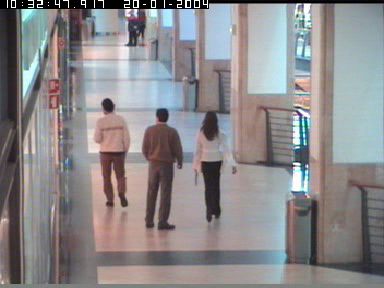
\includegraphics[width=1\textwidth]{dobra_original.png}
\caption{Izvorna slika na kojoj se detektiraju ljudi (dobra detekcija)}
\label{dobra_original}
\end{figure}

\begin{figure}
\centering
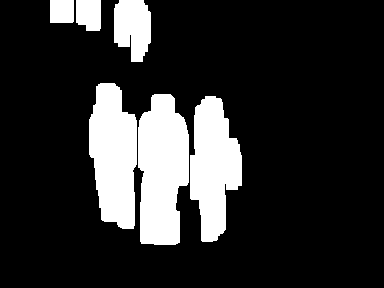
\includegraphics[width=1\textwidth]{dobra_fore.png}
\caption{Binarna slika objekata (dobra detekcija)}
\label{dobra_fore}
\end{figure}

\begin{figure}
\centering
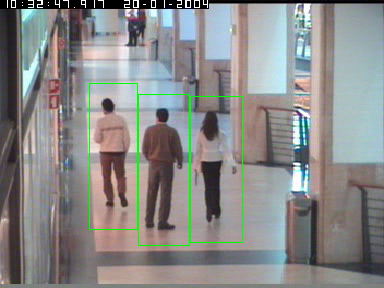
\includegraphics[width=1\textwidth]{dobra_detekt.png}
\caption{Označene osobe (dobra detekcija)}
\label{dobra_detekt}
\end{figure}

%NOVO

\begin{figure}
\centering
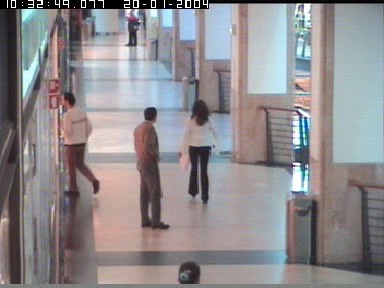
\includegraphics[width=1\textwidth]{lazna_original.png}
\caption{Izvorna slika na kojoj se detektiraju ljudi (lažne detekcije)}
\label{lazna_original}
\end{figure}

\begin{figure}
\centering
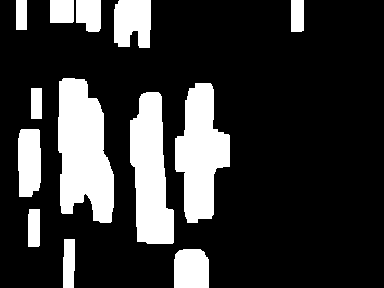
\includegraphics[width=1\textwidth]{lazna_fore.png}
\caption{Binarna slika objekata (lažne detekcije)}
\label{lazna_fore}
\end{figure}

\begin{figure}
\centering
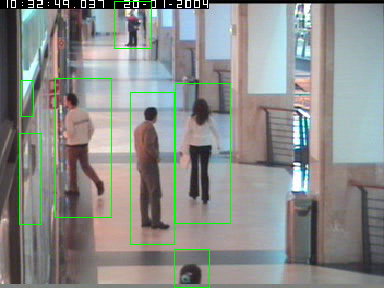
\includegraphics[width=1\textwidth]{lazna_detekt.png}
\caption{Označene osobe (lažne detekcije)}
\label{lazna_detekt}
\end{figure}

%NOVO

\begin{figure}
\centering
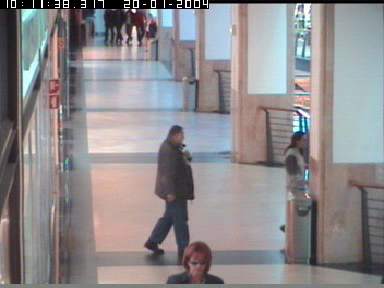
\includegraphics[width=1\textwidth]{otok_original.png}
\caption{Izvorna slika na kojoj se detektiraju ljudi (izostala detekcija)}
\label{otok_original}
\end{figure}

\begin{figure}
\centering
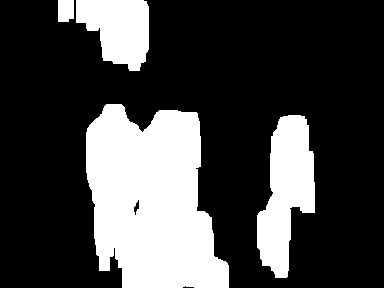
\includegraphics[width=1\textwidth]{otok_fore.png}
\caption{Binarna slika objekata (izostala detekcija)}
\label{otok_fore}
\end{figure}

\begin{figure}
\centering
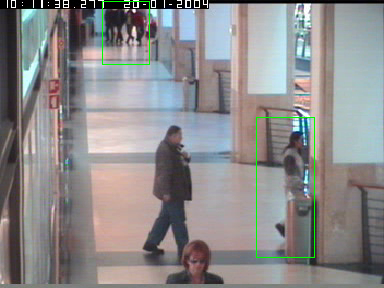
\includegraphics[width=1\textwidth]{otok_detekt.png}
\caption{Označene osobe (izostala detekcija)}
\label{otok_detekt}
\end{figure}


\chapter{Opis programske implementacije rješenja}

\section{Sustav za učenje modela}

Razvijen je programski sustav koji omogućava učenje parametara modela koji služi za detekciju osoba na slikama. Razvijeni sustav sastoji se od četiri modula:

\begin{itemize}

\item Load - modul koji upravljam bazom slika i sadrži funkcije:
\begin{itemize}
	\item loadTrainSet - funkcija koja učitava skup slika za učenje
	\item loadTestSet - funkcija koja učitava skup slika za testiranje
\end{itemize}

	Funkcije vraćaju listu pozitiva(slike na kojima su ljudi) predstavljene kao uređenu dvojku lokacije slike i opisnika slike koji sadrži pozicije osoba na slikama, listu negativa koja sadrži lokaciju negativa


\item Cut - modul koji služi za rezanje slika i sadrži funkcije:
\begin{itemize}
\item getPeople - funkcija koja izrezuje pravokutnike unutar kojih se nalazi osoba na temelju opisnika slike, vraća izrezane pravokutnike
\item getPatches - funkcija koja radi s negativima i nasumično izrezuje dijelove slike, vraća izrezane dijelove slike 
\end{itemize}

\item Extract - modul koji služi za izlučivanje značajki i sastoji se od dva manja modula:
\begin{itemize}
 \item HOG - modul koji služi za računanje HOG opisnika za ulaznu sliku, vraća vektor značajki
 \item Extract - modul koji služi za izlučivanje značajki i sastoji se od dva manja modula:
 \item sastoji se od funkcije getSamples koja pokreće izlučivanje značajki na prethodno izrezanim slikama osoba i nasumičnih dijelova negativa. Svakoj slici dodjeljuje se razred kojemu pripada: 1 - osoba je na slici, 0 - nema osobe na slici. Funkcija vraća matricu značajki i razreda. 
\end{itemize}

\item \emph{train\_hog\_human\_detector.py} - glavni modul koji pokreće učenje detektora te pruža mogućnost provjere naučenog detektora na skupu slika za testiranje.
	Podržava dva moda: učenje i testiranje. Naučeni model sprema se u datoteku. Kod testiranja učitava se model te se provodi testiranje.

\end{itemize}


Unutar glavnog modula moguće je podešavati parametre:
\begin{itemize}
\item veličina pravokutnika na koji se skalira izrezani dio slike (postavljeno 64 x 128)
\item broj nasumičnih dijelova koji se izrezuju iz negativa (postavljeno 3)
\item parametri za HOG opisnik:
\item broj kanala koji se promatraju u histogramu (broj smjerova), (postavljeno 9)
\item broj slikovnih elemenata unutar ćelije (postavljeno 6 x 6)
\item broj ćelija unutar pojedinog bloka (postavljeno 3 x 3)
\item parametri za učenje SVM klasifikatora
\item tip jezgre (postavljena linearna)
\item tip modela (postavljena klasifikacija)
\item broj preklopa u koje se dijeli skup za učenje, radi se k-struka unakrsna provjera (postavljeno k = 3)
\end{itemize}

Naučeni detektor osoba na slikama testira se na skupu slika za testiranje te se za to koristi evaluacijska mjera točnost dobivena na temelju TP, TN, FP, FN klasifikacija. 


\section{Sustav za detekciju}

Za potrebe detekcije i praćenja osoba na slikama razvijen je programski sustav koji se sastoji od šest modula:
\begin{itemize}
	\item Load - modul koji služi za rad s video zapisima i sadrži funkcije:
	\begin{itemize}
		\item load\_video - funkcija koja učitava video 
		\item get\_frames - funkcija koja omogućava generiranje slika iz videa, koristi se funkcija yield čime se omogućeno izravno mijenjanje slike
	\end{itemize}
	
	\item Detection - modul koji radi s naučenim modelom detekcije i sadrži funkciju:
	\begin{itemize}
		\item get\_class - funkcija koja ulaznom objektu dodjeljuje razred kojemu pripada(osoba/nije osoba)
	\end{itemize}
	\item Common - modul koji definira razred SubImage 
	\begin{itemize}
	
	\item sadrži opis podslike: poziciju gornjeg lijevog slikovnog elementa, širinu, visinu te 
			 samu sliku
	\end{itemize}
	
	\item Preprocess - modul koji se bavi obradom slike i sadrži funkcije:
		\begin{itemize}
		\item getRectObjectFromImage - funkcija koja odvaja objekte od pozadine te vraća listu prepoznatih objekata koji dalje idu u detektor osoba
		\item rectIn - funkcija koja prima podatke o pravokutniku i sliku te ispituje nalazi li se neki od kuteva pravokutnika unutar slike 
		\item notContain - funkcija koja prima pravokutnik i skup slika te ispituje nalazi li se ulazni pravokutnik na nekoj od slika 
\end{itemize}

	\item Tracking - modul koji je se bavi praćenjem osoba i sadrži funkciju:
		\begin{itemize}
			\item findSubImages - funkcija prima ulaznu sliku te listu prethodno detektiranih osoba(podslika). 
		  Određuje u koliko se mjeri ulazna slike i promatrana prethodno detektirana osoba poklapaju.
		  Vraća listu osoba koje zadovoljavaju predviđene kriterije poklapanja. 
	\end{itemize}
	
	\item hog\_human\_detection.py - glavni modul koji pokreće detekciju i praćenje osoba na video zapisu
		\begin{itemize}
			\item Povezuje sve prethodno opisane module. 
		\end{itemize}
\end{itemize}

Unutar glavnog modula moguće je postavljati parametre:
\begin{itemize}
	\item odabir naučenog modela koji se koristi za detekciju
	\item veličinu slike koja predstavlja izrezani objekt (veličina mora biti ista kao ona korištena u učenju)
	\item broj slika koji mora proći da bi se ponovno radila detekcija objekata
	\item boju prozora unutar kojeg se nalazi osoba koju pratimo
\end{itemize}

Kriteriji poklapanja određuju se unutar modula Tracking.


\chapter{Zaključak}
Detekcija i praćenje osoba u videosnimkama problem je unutar područja računalnog vida koji svoju primjenu nalazi u raznim područjima od prometa pa sve do uređivanja videa.

U sklopu ovog projekta bilo je potrebno implementirati jedan takav sustav za detekciju i praćenje osoba u videosnimkama. Za opis osoba u slikama korišten je histogram usmjerenih gradijenata, koji se pokazao kao jedna od trenutno najrobusnijih značajki za opis slika. Naučen je model klasifikatora koji koristi te značajke za prepoznavanje ljudi. Implementirani su klasifikator i navedene značajke iskorišteni za detekciju osoba u kompleksnim scenama, te je sve konačno povezano u sustav za praćenje osoba u snimkama.

Eksperimenti su pokazali da realtivno jednostavan linearni klasifikator temeljen na HOG značajkama ima visoku podjednako visoku točnost, preciznost i odziv za pozitivne i negativne primjere. S obzirom da su napravljeni neki kompromisi između brzine rada sustava i iscrpnosti pretraživanja, rezultati rada cjelokupnog sustava nešto su slabiji u kompleksnim scenama na snimkama s dosta šuma u kojima jako varira osvjetljenje. Za snimke s jednostavnom pozadinom sustav radi vrlo dobro. Napravljena je detaljna analiza provedenih eksperimenata i dane su smjernice za buduća poboljšanja.

\bibliography{literatura}
%\bibliographystyle{fer} %promijena za citiranje po redu ieeetr
\bibliographystyle{ieeetr}

\begin{comment}
\begin{sazetak}
Simbolička regresija je postupak otkrivanja matematičkog izraza u skupu podataka. Daje se pregled metoda za simboličku regresiju s naglaskom na genetsko programiranje. Obrađuju se problemi kao što su domene funkcija (nisu definirane na cijelom skupu realnih brojeva). Problemi se rješavaju intervalnom aritmetikom i linearnim skaliranjem. Na kraju se ukratko opisuje mogućnost paralelizacije i primjene. 

\kljucnerijeci{genetsko programiranje, s}

\end{sazetak}

% TODO: Navedite naslov na engleskom jeziku.
\engtitle{Application of graphics coprocessors for program execution on stream programming model}

\begin{abstract}


\keywords{GPU, StreamIt, Sponge, StreamGate, CUDA, stream model, filter, optimization, graphics card}
\end{abstract}
\end{comment}

\end{document}
